\section{Billboard-based visualization}
In this section, we present the work of Ohta et al. \cite{03_billboard}.
The authors use billboard representation to make a 3D model of each player.
This method is simpler than full 3D reconstruction and requires less computation.
A player billboard is a small rectangle standing perpendicular to the ground
and a 2D texture is shown on it.
The difference between 3D reconstruction and billboard representation is shown in Figure \ref{fig:billboard_comparison}:
as we can see, the visual difference is clear at a close viewpoint but becomes very small at a distant one.
For this reason, becomes particularly important to place player billboards at a right place and direction.

\begin{figure}[htbp]
\centerline{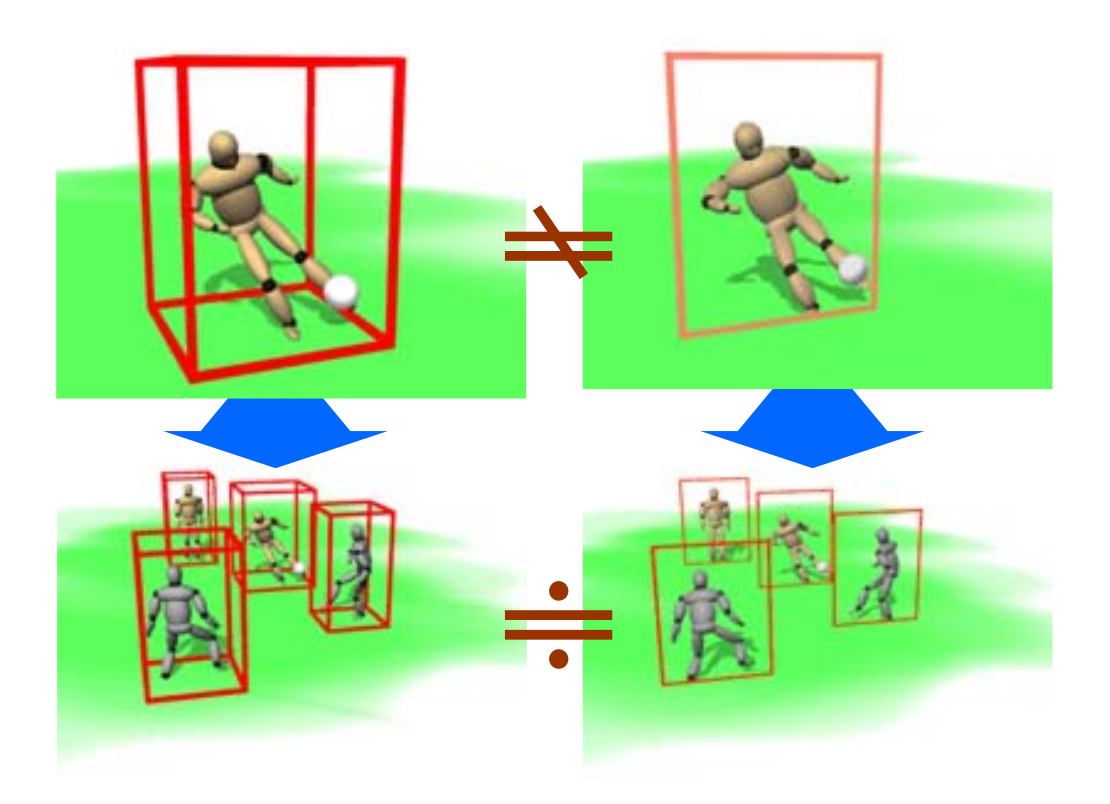
\includegraphics[scale=0.22]{billboard_comparison.png}}
\caption{Appearance similarity between 3D reconstruction and billboard in close and distant view \cite{03_billboard}.}
\label{fig:billboard_comparison}
\end{figure}


The system proceeds as follows: first it extracts texture segments from camera videos, then selects appropriate textures according
to the virtual viewpoint and finally layouts the player billboards in virtual space.

Texture extraction phase consists in obtaining the location of each player and extracting texture segments from every image 
video by projecting player location onto the image plane.
Background region is removed in the texture by video capturing PC.
Please note that camera calibration is done before this phase.

Texture selection phase selects a set of texture to be sent to each viewer based on his viewpoint. 
Given a viewpoint, the system finds the camera that minimizes the angle between the line from the viewpoint to the player 
location and the line from the camera to the player location. Then, a texture segment obtained by that camera is selected 
and placed so that the texture faces the viewpoint \cite{03_billboard}.
% TODO: completare


One problem may happen when players are overlapped each other at a certain camera and billboard texture might include both
of them.
To eliminate extra player region, authors used stereo based method \cite{03_billboard_04} as explained in \cite{03_billboard}. 
% TODO: can be explained more

